%! TEX root = main.tex  % Specifies the main document file for multi-file projects

\chapter{Analysis of a JUCE Project: SARAH Plugin}

The SARAH plugin (Synthèse à Rapide Analyse Harmonique) is an additive synthesizer that operates in the frequency domain. The official documentation and source code are available at:

\begin{itemize}
    \item \url{https://www.getdunne.net/wiki/doku.php?id=sarah}
    \item \url{https://github.com/getdunne/SARAH}
\end{itemize}

\begin{figure}[!htb]
    \centering
    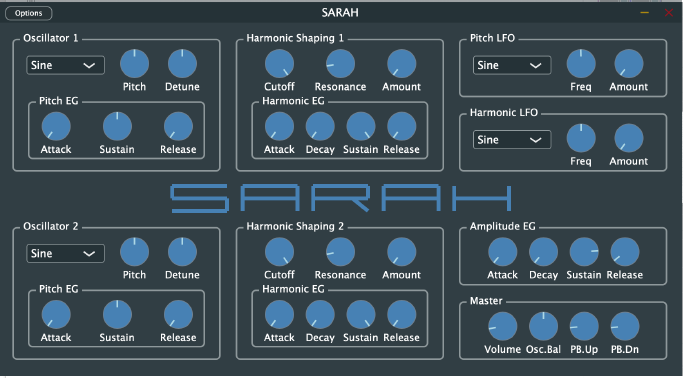
\includegraphics[width=0.8\linewidth]{00_Images/Res/07_chapter/01.png}
    \caption{SARAH plugin}
    \label{fig:sarah}
\end{figure}

\section{Main Features}

SARAH provides the following synthesis and modulation capabilities:

\begin{itemize}
    \item Two oscillators with selectable sinusoidal, square, sawtooth, and triangular waveshapes.
    \item Independent pitch and detuning controls for each oscillator.
    \item Harmonic shaping via frequency-domain filtering.
    \item ADSR amplitude envelope.
    \item ASR pitch envelope.
    \item Low-frequency oscillators (LFOs) for pitch and harmonic modulation.
    \item Global amplitude envelope.
\end{itemize}

\section{Functional Blocks in SARAH}

The plugin can be broken down into three primary functional blocks:

\begin{itemize}
    \item Oscillators: OSC1 and OSC2 generate fundamental audio signals and are instances of the \texttt{SynthOscillator} class.
    \item Low-Frequency Oscillators (LFOs): Used for pitch and harmonic modulation, implemented in the \texttt{SynthLFO} class.
    \item Envelope Generators: ShapeEG1, ShapeEG2, PitchEG1, PitchEG2, and AmpEG, all instances of \texttt{SynthEnvelopeGenerator}.
\end{itemize}

Both \texttt{SynthOscillator} and \texttt{SynthLFO} inherit from the base class \texttt{SynthBaseOscillator}, ensuring a common interface for signal generation.

\begin{figure}[!htb]
    \centering
    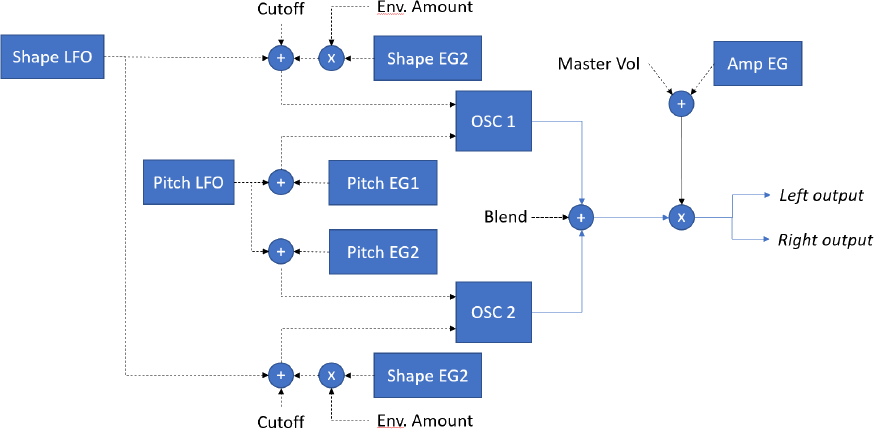
\includegraphics[width=0.7\linewidth]{00_Images/Res/07_chapter/02.png}
    \caption{Functional block}
    \label{fig:functionalblock}
\end{figure}

\section{Wavetable-Based Signal Generation}

\subsection{Wavetable Approach}

The plugin utilizes a wavetable approach for waveform generation. The fundamental concept is:

\begin{itemize}
    \item The square, sawtooth, and triangular waveforms are precomputed and stored in a wavetable.
    \item A fast Fourier transform (FFT) is applied to the waveform to generate its frequency-domain representation.
    \item A harmonic filter is applied, followed by an inverse FFT to reconstruct the waveform.
\end{itemize}

\begin{figure}[!htb]
    \centering
    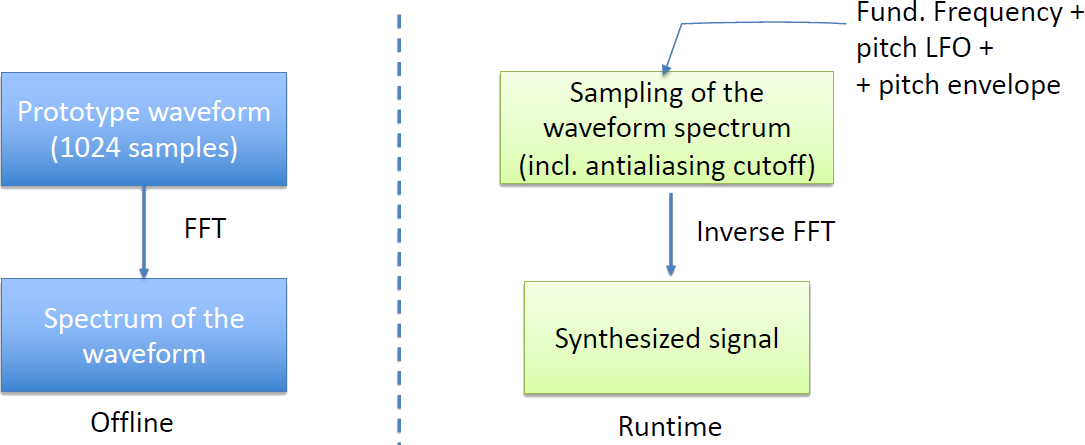
\includegraphics[width=0.6\linewidth]{00_Images/Res/07_chapter/03.png}
    \caption{Wavetable approach}
    \label{fig:wavetableapproach}
\end{figure}

\subsection{Wavetable Formulae}

The synthesized waveforms are generated using the following equations:

\begin{itemize}
    \item Triangle Wave:
    \[
    s(i) = 4 \times (0.5 - | \varphi - 0.5 |) - 1, \quad N = 1024
    \]
    \item Square Wave:
    \[
    s(i) =
    \begin{cases} 
      1 & \text{if } \varphi \leq 0.5 \\
      -1 & \text{if } \varphi > 0.5
    \end{cases}
    \]
    \item Sawtooth Wave:
    \[
    s(i) = 2\varphi - 1
    \]
\end{itemize}

\begin{figure}[!htb]
    \centering
    \subfloat{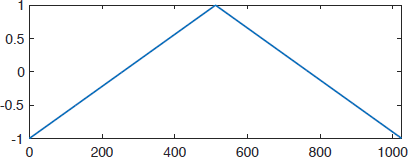
\includegraphics[width=0.3\linewidth]{00_Images/Res/07_chapter/04.png}}\hfill
    \subfloat{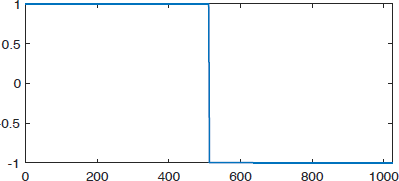
\includegraphics[width=0.3\linewidth]{00_Images/Res/07_chapter/05.png}}\hfill
    \subfloat{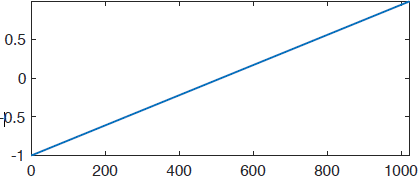
\includegraphics[width=0.3\linewidth]{00_Images/Res/07_chapter/06.png}}
    \caption{Wavetable formulae graphs}
    \label{fig:wavetableformulaegraphs}
\end{figure}

\subsection{Implementation in SARAH}

To generate a waveform at the correct frequency, SARAH follows this approach:

\begin{itemize}
    \item Instead of performing time-domain interpolation, the spectrum of the prototype waveform is sampled and zero-padded.
    \item The actual waveform is generated every time:
    \begin{itemize}
        \item A new note is played.
        \item Pitch is modulated by the LFO.
        \item The plugin starts.
    \end{itemize}
\end{itemize}

\section{Low-Frequency Oscillator (LFO)}

LFOs are used to modulate pitch and harmonic content. The \texttt{SynthLFO} class inherits from \texttt{SynthOscillatorBase} and generates:

\begin{itemize}
    \item Sine waves
    \item Square waves
    \item Triangle waves
    \item Sawtooth waves
\end{itemize}

Unlike audio oscillators, LFOs use a phase-offset technique instead of wavetable interpolation.

\section{Envelope Generator}

\subsection{Purpose of the Envelope Generator}

The \texttt{SynthEnvelopeGenerator} class modulates:

\begin{itemize}
    \item Pitch
    \item Formant filter parameters
    \item Amplitude of the synthesized waveform
\end{itemize}

\subsection{Envelope States}

The envelope has four states:

\begin{itemize}
    \item Idle
    \item Attack
    \item Decay
    \item Sustain
    \item Release
\end{itemize}

SARAH uses the JUCE \texttt{LinearSmoothedValue} class for linear interpolation between values.

\section{Managing Polyphony}

SARAH supports 16 simultaneous voices across 128 program banks. Polyphony is handled using three JUCE classes:

\begin{itemize}
    \item \texttt{Synthesiser}: Manages voices and sound programs.
    \item \texttt{SynthesiserVoice}: Represents a single voice, containing oscillators and envelope generators.
    \item \texttt{SynthesiserSound}: Defines the sound properties assigned to a synthesizer.
\end{itemize}

\subsection{Voice Allocation}

Each new note is assigned to an available voice. The plugin uses an internal voice-stealing mechanism to reallocate voices when necessary.

\section{Audio Processor Integration}

The \texttt{SARAHAudioProcessor} class integrates the synthesizer within the plugin framework. Key functions include:

\begin{itemize}
    \item \texttt{processBlock()}: Processes incoming MIDI messages and generates audio output.
    \item \texttt{getSound()}: Retrieves the current sound settings.
\end{itemize}

\section{Customizing the GUI}

\subsection{JUCE LookAndFeel}

The GUI appearance can be customized using the JUCE \texttt{LookAndFeel} class. This allows:

\begin{itemize}
    \item Customizing colors of UI components.
    \item Redefining how sliders, buttons, and other elements are drawn.
\end{itemize}

\subsection{Example: Custom Rotary Slider}

A rotary slider can be customized by overriding the \texttt{drawRotarySlider} function:

\begin{supercollider*}
void drawRotarySlider (juce::Graphics& g, int x, int y, int width, 
int height, float sliderPos, const float rotaryStartAngle, 
const float rotaryEndAngle, juce::Slider&) override
{
    auto radius = (float) juce::jmin (width / 2, height / 2) - 4.0f;
    auto centreX = (float) x + (float) width  * 0.5f;
    auto centreY = (float) y + (float) height * 0.5f;
    auto angle = rotaryStartAngle + sliderPos * (rotaryEndAngle - rotaryStartAngle);

    g.setColour (juce::Colours::orange);
    g.fillEllipse (centreX - radius, centreY - radius, radius * 2, radius * 2);
}
\end{supercollider*}

\section{Conclusions}

When developing or analyzing a JUCE plugin, it is essential to:

\begin{itemize}
    \item Clearly define the plugin’s purpose and behavior.
    \item Use existing DSP implementations to validate concepts before coding in C++.
    \item Recognize standard plugin architectures to simplify reverse engineering.
\end{itemize}
